% Capítulo gerado a partir de ajuste_de_curvas.tex (arquivos usados neste capítulo)
\def\arqRetaRol{metodo_dos_minimos_quadrados_reta_rolagem.ggb}
\def\arqParabRol{metodo_dos_minimos_quadrados_exemplo02_parabola_rolagem.ggb}
\def\arqAproxRol{aproximacao_funcao_mmq_rolagem.ggb}
\def\arqMMQSimples{01_metodo_dos_minimos_quadrados_linear_simples_TCC_2026.ggb}
\def\arqGDReta{02_RegressaoLinearUsandoGradienteDescendente_junho.ggb}
\def\arqMMQComb{03_metodo_dos_minimos_quadrados_linear_combinada_TCC_2026.ggb}
\def\arqGDPadr{04_aproximacaoGDescCombFuncoespadronizada_03_07.ggb}
\def\arqGDComb{05_aproximacaoGDescCombFuncao.ggb}
\def\arqGDEsc{06_aproximacaoGDescCombFuncao_Escalonada.ggb}
\chapter[Ajuste de curvas]{Ajuste de curvas: método dos mínimos quadrados e gradiente descendente}\label{cap:ajuste}

\begin{tcolorbox}[colback=gray!4,colframe=gray!50,title={Como usar os aplicativos deste capítulo},fonttitle=\bfseries]
Os quadros laranja \emph{Atividade no GeoGebra} trazem o link \textbf{[abrir o aplicativo]}.
São nove aplicativos, em dois grupos.

\textbf{Método direto (sistema normal).}
\begin{itemize}[nosep]
  \item \ggbabrir{\arqRetaRol}{reta com 4 pontos}, \ggbabrir{\arqParabRol}{parábola com 11 pontos} e
        \ggbabrir{\arqAproxRol}{parábola com os pontos $A,\dots,K$}: as contas aparecem passo a passo,
        com barras de rolagem, e o gráfico fica na segunda janela;
  \item \ggbabrir{\arqMMQSimples}{reta com 5 pontos} e
        \ggbabrir{\arqMMQComb}{combinação de $\operatorname{sen}x$, $\cos x$, $x^2$, $x$ e $1$}, montados na planilha.
\end{itemize}

\textbf{Método iterativo (gradiente descendente).}
\begin{itemize}[nosep]
  \item \ggbabrir{\arqGDReta}{reta com 5 pontos}, com as curvas de nível do erro;
  \item \ggbabrir{\arqGDComb}{combinação de funções sem padronizar},
        \ggbabrir{\arqGDEsc}{com as funções padronizadas} e
        \ggbabrir{\arqGDPadr}{padronizadas, com volta aos coeficientes originais}.
\end{itemize}
Nos aplicativos iterativos, o botão de iteração faz um passo do método e o botão \emph{Limpar}
recomeça; o \emph{passo} (taxa de aprendizagem) pode ser alterado na caixa de texto.

Para que os links funcionem, mantenha este PDF e a pasta \texttt{ggb} juntos e abra o PDF num leitor
que permita abrir arquivos externos (Adobe Acrobat Reader, Okular, SumatraPDF, Foxit).
\end{tcolorbox}

% ==================================================================
\section{Interpolar ou ajustar?}

No capítulo de interpolação, procurávamos um polinômio que passasse \emph{exatamente} pelos pontos
dados. Isso nem sempre é desejável:
\begin{itemize}[nosep]
  \item os dados experimentais vêm com erros de medida, e forçar a curva a passar por todos eles
        reproduz também esses erros;
  \item com muitos pontos, o polinômio interpolador tem grau alto e oscila entre os nós;
  \item muitas vezes já se sabe que tipo de função descreve o fenômeno (uma reta, uma parábola, uma
        exponencial) e o que se quer são os seus parâmetros.
\end{itemize}

No \textbf{ajuste de curvas}, escolhemos uma família de funções e procuramos, dentro dela, a que
fica ``mais perto'' dos pontos, sem exigir que passe por eles.

\begin{center}
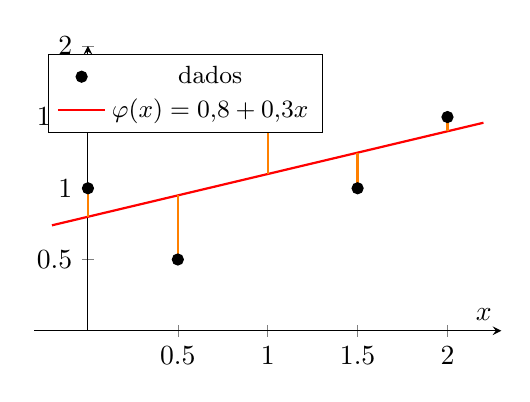
\begin{tikzpicture}
\begin{axis}[width=0.62\textwidth,height=5.2cm,xmin=-0.3,xmax=2.3,ymin=0,ymax=2,
  axis lines=middle,xlabel={$x$},ylabel={$y$},legend pos=north west,legend style={font=\small}]
\addplot[only marks,mark=*,mark size=2pt] coordinates {(0,1) (0.5,0.5) (1,1.5) (1.5,1) (2,1.5)};
\addlegendentry{dados}
\addplot[domain=-0.2:2.2,thick,red] {0.8+0.3*x};
\addlegendentry{$\varphi(x)=0{,}8+0{,}3x$}
\addplot[orange,thick] coordinates {(0,1) (0,0.8)};
\addplot[orange,thick] coordinates {(0.5,0.5) (0.5,0.95)};
\addplot[orange,thick] coordinates {(1,1.5) (1,1.1)};
\addplot[orange,thick] coordinates {(1.5,1) (1.5,1.25)};
\addplot[orange,thick] coordinates {(2,1.5) (2,1.4)};
\end{axis}
\end{tikzpicture}

\small Os segmentos laranja são os resíduos $r_k=f(x_k)-\varphi(x_k)$.
\end{center}

% ==================================================================
\section{O método dos mínimos quadrados (caso discreto)}

São dados $m$ pontos $(x_1,f(x_1)),\dots,(x_m,f(x_m))$ e $n$ funções $g_1(x),\dots,g_n(x)$,
escolhidas conforme o problema. Procuramos
\[
\varphi(x)=\alpha_1g_1(x)+\alpha_2g_2(x)+\dots+\alpha_ng_n(x)
\]
de modo que os \emph{resíduos} $r_k=f(x_k)-\varphi(x_k)$ sejam pequenos. Como resíduos positivos e
negativos se cancelariam numa soma simples, minimizamos a soma dos seus quadrados:
\[
D(\alpha_1,\dots,\alpha_n)=\sum_{k=1}^{m}\big[f(x_k)-\varphi(x_k)\big]^2
=\sum_{k=1}^{m}\Big[f(x_k)-\sum_{j=1}^{n}\alpha_jg_j(x_k)\Big]^2 .
\]
Exemplos de famílias: a reta ($g_1=1$, $g_2=x$), a parábola ($g_1=1$, $g_2=x$, $g_3=x^2$) e a
combinação $\alpha_1\operatorname{sen}x+\alpha_2\cos x+\alpha_3x^2+\alpha_4x+\alpha_5$.

\subsection{O sistema normal}

$D$ é uma função quadrática dos $\alpha_j$, limitada inferiormente por zero. No ponto de mínimo, todas
as derivadas parciais se anulam:
\[
\frac{\partial D}{\partial\alpha_i}=-2\sum_{k=1}^{m}\Big[f(x_k)-\sum_{j=1}^{n}\alpha_jg_j(x_k)\Big]g_i(x_k)=0,
\qquad i=1,\dots,n,
\]
ou seja,
\[
\sum_{j=1}^{n}\Big(\sum_{k=1}^{m}g_i(x_k)g_j(x_k)\Big)\alpha_j=\sum_{k=1}^{m}f(x_k)g_i(x_k),\qquad i=1,\dots,n.
\]

\begin{definicao}[sistema normal]
Com $a_{ij}=\sum_{k=1}^{m}g_i(x_k)g_j(x_k)$ e $b_i=\sum_{k=1}^{m}f(x_k)g_i(x_k)$, os coeficientes
do ajuste são a solução do sistema linear $n\times n$
\[
\begin{bmatrix}a_{11}&\cdots&a_{1n}\\ \vdots&&\vdots\\ a_{n1}&\cdots&a_{nn}\end{bmatrix}
\begin{bmatrix}\alpha_1\\ \vdots\\ \alpha_n\end{bmatrix}=
\begin{bmatrix}b_1\\ \vdots\\ b_n\end{bmatrix}.
\]
A matriz é simétrica ($a_{ij}=a_{ji}$). Se os vetores $(g_j(x_1),\dots,g_j(x_m))$ forem linearmente
independentes, ela é definida positiva, o sistema tem solução única e essa solução é o ponto de mínimo de $D$.
\end{definicao}

Em notação matricial, com $G$ a matriz $m\times n$ de entradas $G_{kj}=g_j(x_k)$ e $\mathbf f=(f(x_1),\dots,f(x_m))^T$,
o sistema normal é $G^TG\,\boldsymbol\alpha=G^T\mathbf f$. É o \textbf{método direto}: monta-se e
resolve-se um sistema linear, por exemplo por eliminação de Gauss (Capítulo~\ref{cap:sistemas}).

\subsection{Ajuste por uma reta}

Para $\varphi(x)=\alpha_1+\alpha_2x$ ($g_1=1$, $g_2=x$), o sistema normal fica
\[
\begin{bmatrix} m & \sum x_k\\ \sum x_k & \sum x_k^2\end{bmatrix}
\begin{bmatrix}\alpha_1\\ \alpha_2\end{bmatrix}=
\begin{bmatrix}\sum f(x_k)\\ \sum x_kf(x_k)\end{bmatrix}.
\]

\begin{exemplo}[{: reta por 5 pontos}]
Os pontos são $(0;1)$, $(0{,}5;\,0{,}5)$, $(1;\,1{,}5)$, $(1{,}5;\,1)$ e $(2;\,1{,}5)$.

\begin{center}
\begin{tabular}{c|rr|rrr}
\toprule
$k$ & $x_k$ & $f(x_k)$ & $g_1g_2=x_k$ & $g_2g_2=x_k^2$ & $fg_2=x_kf(x_k)$\\
\midrule
1 & 0   & 1   & 0   & 0    & 0\\
2 & 0,5 & 0,5 & 0,5 & 0,25 & 0,25\\
3 & 1   & 1,5 & 1   & 1    & 1,5\\
4 & 1,5 & 1   & 1,5 & 2,25 & 1,5\\
5 & 2   & 1,5 & 2   & 4    & 3\\
\midrule
$\sum$ & 5 & 5,5 & 5 & 7,5 & 6,25\\
\bottomrule
\end{tabular}
\end{center}

Como $g_1g_1=1$, $a_{11}=5$. O sistema e a eliminação de Gauss são
\[
\left[\begin{array}{cc|c}5&5&5{,}5\\5&7{,}5&6{,}25\end{array}\right]
\xrightarrow{\;m_{21}=1\;}
\left[\begin{array}{cc|c}5&5&5{,}5\\0&2{,}5&0{,}75\end{array}\right],
\]
logo $\alpha_2=0{,}75/2{,}5=0{,}3$ e $\alpha_1=(5{,}5-5\cdot0{,}3)/5=0{,}8$. Então
$\varphi(x)=0{,}8+0{,}3x$, com $D=\sum r_k^2=0{,}475$.
\end{exemplo}

\begin{atividade}{reta pelo método dos mínimos quadrados}{\arqMMQSimples}
O aplicativo monta na planilha a tabela de $x_k$, $f(x_k)$, $g_1(x_k)=1$, $g_2(x_k)=x_k$, dos produtos
$g_ig_j$ e $fg_i$ e das somas, e resolve o sistema normal por eliminação de Gauss ($m_{21}$, $\alpha_2$,
$\alpha_1$). A reta $\varphi$ aparece no gráfico com os pontos $A_0,\dots,A_4$.

\textbf{Tarefas.} (a) Confira a tabela e a reta do exemplo. (b) Mova um ponto para longe dos demais
(um \emph{dado discrepante}) e observe quanto a reta se desloca. (c) Alinhe os cinco pontos numa reta:
qual é então o valor de $D$?
\end{atividade}

\begin{atividade}{reta com rolagem (4 pontos)}{\arqRetaRol}
Todas as etapas aparecem em textos na janela da esquerda, com barras de rolagem: tabela dos produtos,
sistema normal, eliminação de Gauss, substituição regressiva, tabela de resíduos e comparação com a
parábola. Na janela da direita estão os pontos (que podem ser arrastados), a reta, os resíduos e a
conferência com o comando \texttt{FitPoly} do GeoGebra. Com os pontos iniciais,
$\varphi(x)=1{,}0735+0{,}2941x$.

\textbf{Tarefas.} (a) Gere pontos aleatórios e compare $D$ para a reta e para a parábola.
(b) Explique por que o $D$ da parábola nunca é maior que o da reta.
\end{atividade}

\subsection{Ajuste por uma parábola}

Para $\varphi(x)=\alpha_1+\alpha_2x+\alpha_3x^2$ ($g_1=1$, $g_2=x$, $g_3=x^2$):
\[
\begin{bmatrix} m & \sum x_k & \sum x_k^2\\ \sum x_k & \sum x_k^2 & \sum x_k^3\\ \sum x_k^2 & \sum x_k^3 & \sum x_k^4\end{bmatrix}
\begin{bmatrix}\alpha_1\\ \alpha_2\\ \alpha_3\end{bmatrix}=
\begin{bmatrix}\sum f(x_k)\\ \sum x_kf(x_k)\\ \sum x_k^2f(x_k)\end{bmatrix}.
\]

\begin{atividade}{parábola com 11 pontos}{\arqParabRol}
Mesmo formato do aplicativo da reta, agora com $g_3(x)=x^2$, três multiplicadores ($m_{21}$, $m_{31}$,
$m_{32}$) e os pontos $A_0,\dots,A_{10}$, dispostos em forma de ``U''. O resultado inicial é
$\varphi(x)=0{,}2144+0{,}4555x+1{,}8492x^2$.

\textbf{Tarefas.} (a) Compare o $R^2$ da parábola e o da reta: qual modelo descreve melhor esses dados?
(b) Use o campo ``avaliar $\varphi$ em $x$'' para estimar o valor em $x=1{,}2$, fora do intervalo dos
dados (extrapolação). Que cuidado se deve ter?
\end{atividade}

\begin{atividade}{parábola com os pontos $A,\dots,K$}{\arqAproxRol}
Outro conjunto de 11 pontos, agora mais espalhados. O ajuste é
$\varphi(x)=0{,}7873-0{,}1454x+0{,}2068x^2$, com $D\approx2{,}06$ e $R^2\approx0{,}77$, contra
$D\approx7{,}86$ e $R^2\approx0{,}11$ da reta.

\textbf{Tarefa.} Mostre os resíduos e identifique o ponto que mais contribui para $D$.
\end{atividade}

\subsection{Combinação de outras funções}

O método não exige polinômios. Basta que $\varphi$ seja \emph{linear nos parâmetros}.

\begin{exemplo}[{: $\varphi(x)=\alpha_1\operatorname{sen}x+\alpha_2\cos x+\alpha_3x^2+\alpha_4x+\alpha_5$}]\label{ex:comb}
Os 8 pontos são
\[
(-2;2),\ (0;0),\ (4;2),\ (8;0),\ (10;5),\ (14;4),\ (16;8),\ (20;10).
\]
O sistema normal é $5\times5$, com $g_1=\operatorname{sen}x$, $g_2=\cos x$, $g_3=x^2$, $g_4=x$ e $g_5=1$:
\[
\begin{bmatrix}
4{,}572 & 1{,}969 & 478{,}80 & 28{,}787 & 0{,}395\\
1{,}969 & 3{,}428 & -160{,}47 & -16{,}584 & -1{,}467\\
478{,}80 & -160{,}47 & 278\,320 & 16\,408 & 1\,036\\
28{,}787 & -16{,}584 & 16\,408 & 1\,036 & 70\\
0{,}395 & -1{,}467 & 1\,036 & 70 & 8
\end{bmatrix}
\begin{bmatrix}\alpha_1\\ \alpha_2\\ \alpha_3\\ \alpha_4\\ \alpha_5\end{bmatrix}=
\begin{bmatrix}4{,}736\\ -9{,}368\\ 7\,372\\ 438\\ 31\end{bmatrix}.
\]
A solução é
\[
\varphi(x)\approx-2{,}2594\operatorname{sen}x+0{,}1701\cos x+0{,}02518x^2+0{,}09374x-0{,}06376,
\qquad D\approx0{,}5606 .
\]
Repare na diferença de escala entre as entradas: $4{,}6$ na diagonal para $\operatorname{sen}x$ e
$278\,320$ para $x^2$. Ela não atrapalha o método direto, mas, como veremos, prejudica muito o gradiente descendente.
\end{exemplo}

\begin{center}
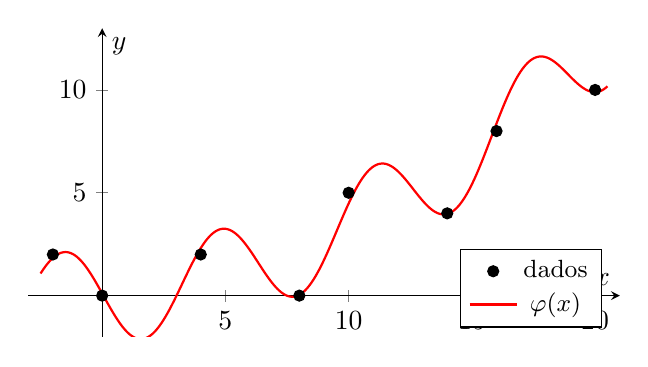
\begin{tikzpicture}
\begin{axis}[width=0.75\textwidth,height=5.5cm,xmin=-3,xmax=21,ymin=-2,ymax=13,axis lines=middle,
  xlabel={$x$},ylabel={$y$},legend pos=south east,legend style={font=\small}]
\addplot[only marks,mark=*,mark size=2pt] coordinates {(-2,2) (0,0) (4,2) (8,0) (10,5) (14,4) (16,8) (20,10)};
\addlegendentry{dados}
\addplot[domain=-2.5:20.5,samples=300,thick,red] {-2.259395*sin(deg(x))+0.17013*cos(deg(x))+0.025184*x^2+0.093738*x-0.063763};
\addlegendentry{$\varphi(x)$}
\end{axis}
\end{tikzpicture}
\end{center}

\begin{atividade}{combinação de funções pelo método direto}{\arqMMQComb}
A planilha calcula os produtos $g_ig_j$ e $fg_i$ para as cinco funções, as somas que formam o sistema
normal $5\times5$, os multiplicadores da eliminação de Gauss e os coeficientes $\alpha_1,\dots,\alpha_5$
por substituição regressiva.

\textbf{Tarefas.} (a) Confira os valores do Exemplo~\ref{ex:comb}. (b) Retire a função $\operatorname{sen}x$
(isto é, ajuste só com $\cos x$, $x^2$, $x$ e $1$). O ajuste piora muito? Por quê?
\end{atividade}

\subsection{Casos não lineares: linearização}

Se $\varphi$ não é linear nos parâmetros, às vezes uma mudança de variáveis resolve. Para
$\varphi(x)=a\,e^{bx}$, tomando logaritmos:
\[
z=\ln\varphi(x)=\ln a+bx=\alpha_1+\alpha_2x,
\]
e ajustamos uma reta aos pontos $(x_k,\ln f(x_k))$. Com os dados
\begin{center}\small
\begin{tabular}{c|cccccccc}
$x_k$ & $-1$ & $-0{,}7$ & $-0{,}4$ & $-0{,}1$ & $0{,}2$ & $0{,}5$ & $0{,}8$ & $1$\\ \hline
$f(x_k)$ & 36,547 & 17,264 & 8,155 & 3,852 & 1,820 & 0,860 & 0,406 & 0,246
\end{tabular}
\end{center}
obtemos $\alpha_1\approx1{,}0986$ e $\alpha_2\approx-2{,}5002$, logo $a=e^{\alpha_1}\approx3{,}0$ e
$\varphi(x)\approx3{,}0\,e^{-2{,}5x}$.

\begin{observacao}
O ajuste linearizado minimiza os quadrados dos resíduos de $\ln f$, e não os de $f$. O resultado é bom,
mas não é exatamente o mínimo de $\sum[f(x_k)-a e^{bx_k}]^2$. Para esse mínimo, é preciso um método
iterativo, como o gradiente descendente da próxima seção.
\end{observacao}

% ==================================================================
\section{O método iterativo: gradiente descendente}

Em vez de igualar o gradiente a zero e resolver um sistema, podemos \emph{caminhar} em direção ao mínimo.
O gradiente de uma função aponta na direção de maior crescimento; andando no sentido oposto, a função
diminui. É a ideia do \textbf{gradiente descendente}, o método usado para treinar modelos de regressão
e redes neurais em aprendizado de máquina.

\subsection{A função custo e o seu gradiente}

Nos aplicativos, o erro é escrito com os resíduos no sentido do modelo, $e_k=\varphi(x_k)-f(x_k)$, e
dividido por $2m$, como é costume em aprendizado de máquina:
\[
J(\boldsymbol\alpha)=\frac{1}{2m}\sum_{k=1}^{m}e_k^2=\frac{1}{2m}\sum_{k=1}^{m}\Big[\sum_{j=1}^{n}\alpha_jg_j(x_k)-f(x_k)\Big]^2=\frac{D(\boldsymbol\alpha)}{2m}.
\]
Como $J$ é um múltiplo positivo de $D$, os dois têm o mesmo ponto de mínimo. As derivadas parciais são
\[
\frac{\partial J}{\partial\alpha_j}=\frac1m\sum_{k=1}^{m}e_k\,g_j(x_k),\qquad j=1,\dots,n .
\]

\begin{tcolorbox}[colback=azul!3,colframe=azul!60,title={Algoritmo: gradiente descendente},fonttitle=\bfseries]
\begin{description}[nosep,font=\normalfont\bfseries]
  \item[Passo 0:] escolha $\boldsymbol\alpha^{(0)}$ (por exemplo, zero), o passo $\eta>0$, a tolerância e o número máximo de iterações.
  \item[Passo 1:] calcule os resíduos $e_k=\varphi(x_k)-f(x_k)$ com os coeficientes atuais.
  \item[Passo 2:] calcule o gradiente $d_j=\frac1m\sum_k e_k\,g_j(x_k)$, $j=1,\dots,n$.
  \item[Passo 3:] atualize todos os coeficientes \emph{simultaneamente}: $\alpha_j^{(i+1)}=\alpha_j^{(i)}-\eta\,d_j$.
  \item[Passo 4:] se $\|\mathbf d\|$ (ou a variação de $J$) for menor que a tolerância, pare; caso contrário, volte ao passo 1.
\end{description}
\end{tcolorbox}

O passo $\eta$ é chamado \emph{taxa de aprendizagem}. Nos aplicativos, a atualização simultânea é feita
guardando os valores antigos (\texttt{a1\_antigo}, \texttt{d1\_antigo}, \dots) antes de alterar os coeficientes.

\subsection{Gradiente descendente para a reta}\label{sec:gdreta}

No aplicativo da reta, o modelo é $\varphi(x)=\alpha_1x+\alpha_2$ (aqui $\alpha_1$ é a inclinação e
$\alpha_2$ o termo independente) e
\[
\frac{\partial J}{\partial\alpha_1}=\frac1m\sum e_kx_k,\qquad \frac{\partial J}{\partial\alpha_2}=\frac1m\sum e_k .
\]

\begin{exemplo}[{: as primeiras iterações, com $\eta=0{,}1$ e os 5 pontos do exemplo anterior}]
Começando de $\alpha_1=\alpha_2=0$, os resíduos são $e=(-1;\,-0{,}5;\,-1{,}5;\,-1;\,-1{,}5)$, e então
\[
\frac{\partial J}{\partial\alpha_1}=\frac{0-0{,}25-1{,}5-1{,}5-3}{5}=-1{,}25,\qquad
\frac{\partial J}{\partial\alpha_2}=\frac{-5{,}5}{5}=-1{,}1,
\]
\[
\alpha_1^{(1)}=0-0{,}1(-1{,}25)=0{,}125,\qquad \alpha_2^{(1)}=0-0{,}1(-1{,}1)=0{,}11 .
\]
Continuando:

\begin{center}
\begin{tabular}{rccc}
\toprule
iteração & $\alpha_1$ (inclinação) & $\alpha_2$ (termo indep.) & $D=\sum e_k^2$\\
\midrule
0 & 0 & 0 & 6,75\\
1 & 0,125 & 0,11 & 4,2927\\
2 & 0,22025 & 0,1965 & 2,8251\\
3 & 0,29256 & 0,26483 & 1,9473\\
10 & 0,47673 & 0,48470 & 0,6491\\
50 & 0,39059 & 0,68397 & 0,4988\\
100 & 0,32991 & 0,76170 & 0,4776\\
500 & 0,30000 & 0,79999 & 0,4750\\
\bottomrule
\end{tabular}
\end{center}

O método converge para $\alpha_1=0{,}3$ e $\alpha_2=0{,}8$, a mesma reta $\varphi(x)=0{,}3x+0{,}8$ do método direto,
mas precisou de algumas centenas de iterações.
\end{exemplo}

\begin{center}
\begin{tikzpicture}
\begin{axis}[width=0.46\textwidth,height=5.2cm,xlabel={iteração},ylabel={$J$},
  title={\small $J$ ao longo das iterações ($\eta=0{,}1$)},xmin=0,xmax=300,ymin=0,ymax=0.7,
  yticklabel style={/pgf/number format/fixed,/pgf/number format/use comma}]
\addplot[thick,azul] coordinates {(0,0.675) (1,0.429269) (2,0.282505) (3,0.194728) (4,0.142113) (5,0.110462) (6,0.0913175) (7,0.0796366) (8,0.072415) (9,0.0678619) (10,0.0649096) (20,0.0565007) (30,0.0532653) (40,0.0512007) (50,0.0498754) (60,0.0490248) (70,0.0484788) (80,0.0481283) (90,0.0479033) (100,0.0477589) (120,0.0476067) (140,0.0475439) (160,0.0475181) (200,0.0475031) (250,0.0475003) (300,0.0475)};
\end{axis}
\end{tikzpicture}\hfill
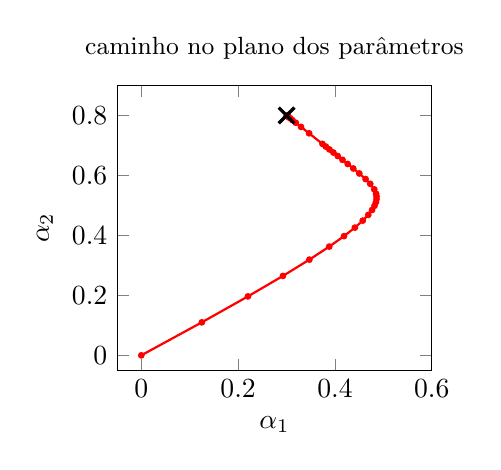
\begin{tikzpicture}
\begin{axis}[width=0.46\textwidth,height=5.2cm,xlabel={$\alpha_1$},ylabel={$\alpha_2$},
  title={\small caminho no plano dos parâmetros},xmin=-0.05,xmax=0.6,ymin=-0.05,ymax=0.9]
\addplot[thick,red,mark=*,mark size=0.8pt] coordinates {(0.0000,0.0000) (0.1250,0.1100) (0.2203,0.1965) (0.2926,0.2648) (0.3472,0.3191) (0.3882,0.3625) (0.4187,0.3974) (0.4412,0.4258) (0.4574,0.4491) (0.4689,0.4684) (0.4767,0.4847) (0.4817,0.4986) (0.4846,0.5105) (0.4859,0.5210) (0.4859,0.5303) (0.4850,0.5387) (0.4812,0.5534) (0.4729,0.5718) (0.4633,0.5877) (0.4503,0.6064) (0.4379,0.6231) (0.4263,0.6381) (0.4156,0.6519) (0.4058,0.6645) (0.3968,0.6760) (0.3886,0.6865) (0.3811,0.6961) (0.3742,0.7050) (0.3466,0.7403) (0.3299,0.7617) (0.3192,0.7754) (0.3123,0.7842) (0.3079,0.7899) (0.3051,0.7935) (0.3033,0.7958) (0.3021,0.7973) (0.3013,0.7983) (0.3009,0.7989) (0.3004,0.7995)};
\addplot[only marks,mark=x,mark size=4pt,very thick] coordinates {(0.3,0.8)};
\end{axis}
\end{tikzpicture}
\end{center}

\begin{atividade}{regressão linear por gradiente descendente}{\arqGDReta}
Os pontos são $J$, $K$, $L$, $M$ e $T$, os mesmos do exemplo. O botão \textbf{Iteração} faz um passo do
método; \textbf{Limpar os Dados} volta a $\alpha_1=\alpha_2=0$. O aplicativo mostra:
\begin{itemize}[nosep]
  \item a reta $\varphi$, os resíduos e o erro $\text{SSE}=\sum e_k^2$;
  \item as tabelas de $x_k$, $y_k$ e $\hat y_k=\varphi(x_k)$;
  \item as curvas de nível do erro no plano $(\alpha_1,\alpha_2)$ (elipses), com o ponto $(\alpha_1,\alpha_2)$
        caminhando em direção ao centro.
\end{itemize}
\textbf{Tarefas.} (a) Faça 10 iterações e confira a tabela do exemplo ($\alpha_1\approx0{,}4767$,
$\alpha_2\approx0{,}4847$). (b) Observe que o caminho é sempre perpendicular às curvas de nível.
(c) Repita com $\eta=0{,}5$ e $\eta=0{,}85$. (d) Tente $\eta=0{,}9$: o que acontece?
\end{atividade}

\subsection{A escolha do passo e a convergência}

Como $J$ é quadrática, $J(\boldsymbol\alpha)=J(\boldsymbol\alpha^*)+\tfrac12(\boldsymbol\alpha-\boldsymbol\alpha^*)^TH(\boldsymbol\alpha-\boldsymbol\alpha^*)$,
com $H=\frac1mG^TG$ (a matriz do sistema normal dividida por $m$). A iteração fica
\[
\boldsymbol\alpha^{(i+1)}-\boldsymbol\alpha^*=(I-\eta H)\,(\boldsymbol\alpha^{(i)}-\boldsymbol\alpha^*).
\]
É uma iteração de ponto fixo, como as do Capítulo~\ref{cap:zeros} e os métodos iterativos do
Capítulo~\ref{cap:sistemas}. Se $\lambda_{\min}$ e $\lambda_{\max}$ são o menor e o maior autovalor de $H$:
\begin{itemize}[nosep]
  \item o método converge se, e somente se, $0<\eta<2/\lambda_{\max}$;
  \item mesmo com o melhor passo, o erro cai por um fator próximo de
        $\dfrac{\kappa-1}{\kappa+1}$ por iteração, onde $\kappa=\lambda_{\max}/\lambda_{\min}$ é o
        \emph{número de condição} de $H$. Quanto maior $\kappa$, mais lenta a convergência.
\end{itemize}

No exemplo da reta, os autovalores de $H$ são $0{,}219$ e $2{,}281$. O passo máximo é
$2/2{,}281\approx0{,}877$ (por isso $\eta=0{,}9$ diverge) e $\kappa\approx10{,}4$.

\subsection{Padronização das variáveis}

No Exemplo~\ref{ex:comb}, os autovalores de $H$ vão de $0{,}051$ a $34\,912$, e $\kappa\approx6{,}8\times10^{5}$.
O passo máximo é $2/34\,912\approx5{,}7\times10^{-5}$. Com um passo tão pequeno, os coeficientes de
$\operatorname{sen}x$, $\cos x$ e $1$ quase não se movem: a função $x^2$, com valores até 400, domina o gradiente.

A solução é \textbf{padronizar} cada função: subtrair a média e dividir pelo desvio padrão dos seus valores nos pontos,
\[
\tilde g_j(x)=\frac{g_j(x)-\mu_j}{\sigma_j},\qquad
\mu_j=\frac1m\sum_kg_j(x_k),\quad \sigma_j=\sqrt{\frac1m\sum_k\big(g_j(x_k)-\mu_j\big)^2},
\]
e ajustar $\varphi(x)=\beta_1\tilde g_1(x)+\dots+\beta_4\tilde g_4(x)+\beta_5$. Agora todas as funções
têm média 0 e desvio 1 nos pontos. O número de condição cai para $\kappa\approx102$, e o passo pode ser
$\eta=0{,}1$. Como as $\tilde g_j$ têm média zero, a derivada em relação a $\beta_5$ fica
$\frac1m\sum e_k=0$ quando $\beta_5=\bar f$: por isso os aplicativos começam com $\beta_5$ igual à média dos $y_k$.

Os coeficientes originais são recuperados por
\[
\alpha_j=\frac{\beta_j}{\sigma_j}\quad(j=1,\dots,4),\qquad
\alpha_5=\beta_5-\sum_{j=1}^{4}\frac{\beta_j\mu_j}{\sigma_j}.
\]

\begin{exemplo}[{: sem e com padronização}]
Para os dados do Exemplo~\ref{ex:comb}, partindo de coeficientes nulos ($\beta_5=\bar f=3{,}875$ no caso padronizado):

\begin{center}
\begin{tabular}{rcc}
\toprule
iteração & $J$ sem padronizar ($\eta=10^{-6}$) & $J$ padronizado ($\eta=0{,}1$)\\
\midrule
0    & 13,3125 & 5,8047\\
10   & 7,1039  & 0,8488\\
50   & 1,4570  & 0,1217\\
100  & 1,1176  & 0,0476\\
500  & 1,1069  & 0,0361\\
1000 & 1,1060  & 0,0351\\
5000 & 1,0990  & 0,03504\\
\bottomrule
\end{tabular}
\end{center}

O mínimo é $J=D/16\approx0{,}03504$. Sem padronizar, depois de 5000 iterações o erro ainda é 30 vezes maior;
com padronização, o método chega ao mínimo e os $\beta_j$ convertidos dão os mesmos $\alpha_j$ do método direto.
\end{exemplo}

\begin{center}
\begin{tikzpicture}
\begin{axis}[width=0.7\textwidth,height=5.5cm,xlabel={iteração},ylabel={$J$},xmode=log,ymode=log,
  legend style={font=\small,at={(0.5,1.03)},anchor=south},legend columns=2,xmin=1,xmax=5000]
\addplot[thick,red,mark=*,mark size=1pt] coordinates {(1,12.4752) (2,11.6953) (5,9.66234) (10,7.10386) (20,4.05357) (50,1.45697) (100,1.11755) (200,1.10738) (500,1.10685) (1000,1.10597) (2000,1.10422) (5000,1.09902)};
\addlegendentry{sem padronizar, $\eta=10^{-6}$}
\addplot[thick,azul,mark=*,mark size=1pt] coordinates {(1,4.11939) (2,3.04881) (5,1.56211) (10,0.84876) (20,0.446914) (50,0.121745) (100,0.0475599) (200,0.0396608) (500,0.0361489) (1000,0.0351439) (2000,0.0350413) (5000,0.0350404)};
\addlegendentry{padronizado, $\eta=0{,}1$}
\addplot[dashed,gray,domain=1:5000] {0.03504};
\addlegendentry{mínimo (método direto)}
\end{axis}
\end{tikzpicture}
\end{center}

\begin{atividade}{combinação de funções sem padronizar}{\arqGDComb}
Funções $\varphi_1=\operatorname{sen}x$, $\varphi_2=\cos x$, $\varphi_3=x^2$, $\varphi_4=x$ e $\varphi_5=1$,
os mesmos 8 pontos do Exemplo~\ref{ex:comb} e o passo $10^{-6}$. O botão de iteração aplica um passo; o campo
\texttt{iter} conta as iterações e o texto mostra o erro $J$ e os parâmetros.

\textbf{Tarefas.} (a) Faça 50 iterações e confira $J\approx1{,}457$. (b) Aumente o passo para $10^{-4}$ e
observe a divergência ($10^{-4}>5{,}7\times10^{-5}$). (c) Compare os parâmetros com os do método direto.
\end{atividade}

\begin{atividade}{combinação de funções padronizadas}{\arqGDEsc}
As funções são padronizadas pela média e pelo desvio padrão dos seus valores nos pontos
(\texttt{medsen}, \texttt{desvsen}, \dots), e $\beta_5$ começa igual à média dos $y_k$. O passo é $0{,}1$.

\textbf{Tarefas.} (a) Com 9 iterações, confira $J\approx0{,}931$. (b) Continue até $J$ estabilizar perto de
$0{,}035$. (c) Verifique que a derivada em relação a $\beta_5$ fica praticamente nula.
\end{atividade}

\begin{atividade}{padronizado, com volta aos coeficientes originais}{\arqGDPadr}
Mesmo ajuste, com passo $0{,}01$ e controles deslizantes para $\beta_1,\dots,\beta_4$ (também se pode
procurar o mínimo ``à mão''). O aplicativo calcula $\alpha_j=\beta_j/\sigma_j$ e
$\alpha_5=\beta_5-\sum\beta_j\mu_j/\sigma_j$.

\textbf{Tarefa.} Depois de convergir, compare os $\alpha_j$ com os do aplicativo do método direto
(\ggbabrir{\arqMMQComb}{combinação de funções}).
\end{atividade}

% ==================================================================
\section{Método direto \texorpdfstring{$\times$}{x} método iterativo}

\begin{center}
\small
\begin{tabular}{p{3.2cm}p{5.2cm}p{5.2cm}}
\toprule
 & método direto (sistema normal) & gradiente descendente\\
\midrule
ideia & igualar o gradiente a zero e resolver $G^TG\boldsymbol\alpha=G^T\mathbf f$ & caminhar contra o gradiente: $\boldsymbol\alpha\leftarrow\boldsymbol\alpha-\eta\nabla J$\\
resultado & exato (a menos de arredondamento) em número finito de operações & aproximação que melhora a cada iteração\\
custo & montar $G^TG$ e resolver um sistema $n\times n$ (cerca de $n^3/3$ operações) & cada iteração custa da ordem de $mn$ operações\\
parâmetros & nenhum & passo $\eta$, chute inicial, critério de parada\\
sensibilidade & mal condicionamento de $G^TG$ afeta a precisão & mal condicionamento deixa a convergência lenta; padronizar ajuda\\
quando usar & poucos parâmetros, modelo linear nos parâmetros & muitos dados ou parâmetros, modelos não lineares, redes neurais\\
\bottomrule
\end{tabular}
\end{center}

\begin{observacao}
Os dois métodos minimizam a mesma função. Para modelos lineares nos parâmetros e poucos coeficientes, o método
direto é o mais simples e preciso. O gradiente descendente mostra a sua força quando o sistema normal é grande
demais para ser montado, ou quando o modelo não é linear nos parâmetros (por exemplo, $a\,e^{bx}$ sem
linearizar, ou uma rede neural). Nesses casos não há sistema linear a resolver, mas o gradiente continua
disponível.
\end{observacao}

% ==================================================================
\section{Exercícios}

\begin{enumerate}[label=\arabic*.]
  \item Ajuste uma reta aos pontos $(1;\,2)$, $(2;\,3)$, $(3;\,5)$ e $(4;\,6)$ pelo sistema normal e calcule $D$.
  \item Para os mesmos pontos, faça duas iterações do gradiente descendente com $\varphi(x)=\alpha_1x+\alpha_2$,
        $\eta=0{,}05$, partindo de $\alpha_1=\alpha_2=0$.
  \item Mostre que, para a reta, a primeira equação do sistema normal equivale a $\bar f=\alpha_1+\alpha_2\bar x$:
        a reta de mínimos quadrados passa pelo ponto médio $(\bar x,\bar f)$.
  \item Escreva o sistema normal para $\varphi(x)=\alpha_1+\alpha_2\cos x$.
  \item Linearize $\varphi(x)=a\,x^{b}$ e $\varphi(x)=\dfrac{1}{a+bx}$.
  \item No exemplo da Seção~\ref{sec:gdreta}, os autovalores de $H$ são $0{,}219$ e $2{,}281$. Qual o maior passo
        que garante convergência? Que passo dá a convergência mais rápida?
  \item Explique por que, depois de padronizar as funções $g_1,\dots,g_4$, a derivada de $J$ em relação ao termo
        constante $\beta_5$ se anula quando $\beta_5=\bar f$, quaisquer que sejam $\beta_1,\dots,\beta_4$.
\end{enumerate}

\subsection*{Respostas}
\begin{enumerate}[label=\arabic*.,nosep]
  \item $\sum x=10$, $\sum x^2=30$, $\sum f=16$, $\sum xf=47$. O sistema é $4\alpha_1+10\alpha_2=16$,
        $10\alpha_1+30\alpha_2=47$, com solução $\alpha_1=0{,}5$, $\alpha_2=1{,}4$, logo $\varphi(x)=0{,}5+1{,}4x$ e $D=0{,}2$.
  \item Iteração 1: $e=(-2,-3,-5,-6)$, gradientes $-11{,}75$ e $-4$, logo $\alpha_1=0{,}5875$, $\alpha_2=0{,}2$.
        Iteração 2: $e=(-1{,}2125;\,-1{,}625;\,-3{,}0375;\,-3{,}45)$, gradientes $-6{,}84375$ e $-2{,}33125$, logo
        $\alpha_1\approx0{,}92969$, $\alpha_2\approx0{,}31656$.
  \item Dividindo $m\alpha_1+\alpha_2\sum x_k=\sum f(x_k)$ por $m$.
  \item $\begin{bmatrix} m & \sum\cos x_k\\ \sum\cos x_k & \sum\cos^2x_k\end{bmatrix}\begin{bmatrix}\alpha_1\\ \alpha_2\end{bmatrix}=\begin{bmatrix}\sum f(x_k)\\ \sum f(x_k)\cos x_k\end{bmatrix}$.
  \item $\ln\varphi=\ln a+b\ln x$ (reta nos pontos $(\ln x_k,\ln f(x_k))$); $1/\varphi=a+bx$ (reta nos pontos $(x_k,1/f(x_k))$).
  \item $\eta<2/2{,}281\approx0{,}877$. O passo ótimo é $2/(\lambda_{\min}+\lambda_{\max})=2/2{,}5=0{,}8$.
  \item $\partial J/\partial\beta_5=\frac1m\sum e_k=\frac1m\sum_k\big(\sum_j\beta_j\tilde g_j(x_k)+\beta_5-f(x_k)\big)
        =\sum_j\beta_j\overline{\tilde g_j}+\beta_5-\bar f=\beta_5-\bar f$, pois cada $\tilde g_j$ tem média zero.
\end{enumerate}

\subsection*{Referências}
\begin{itemize}[nosep]
  \item M.~A.~G.~Ruggiero e V.~L.~R.~Lopes, \emph{Cálculo Numérico: aspectos teóricos e computacionais}, 2.ª ed., Makron Books (cap.~6, ajuste de curvas).
  \item A.~Géron, \emph{Mãos à obra: aprendizado de máquina com Scikit-Learn, Keras e TensorFlow}, Alta Books (gradiente descendente e padronização).
\end{itemize}
